\documentclass[final]{beamer} % use beamer

%\usepackage[usenames,dvipsnames]{xcolor}
\usepackage[orientation=portrait,size=a0,scale=1.6]{beamerposter}
\usepackage[english]{babel}
\usepackage[utf8]{inputenc}
\usepackage{amsfonts}
\usepackage{amsthm}
\usepackage{amsmath}
\usepackage{pgf}
\usepackage{palatino}
\usepackage{comment}
\usepackage{natbib}
\usepackage{paralist}
\usepackage{epstopdf}
\usepackage{algorithm}
\usepackage{caption}
\usepackage{algorithmic}
\usepackage{tcolorbox}
\usepackage{mathtools} % MoveEqLeft
\setbeamertemplate{bibliography item}[text]

\setlength{\leftmargini}{2cm}


%\usetheme{bpiresicml2013}
\usepackage{beamerthemebpiresicml2013}

%\setbeamercolor{block title}{fg=black,bg=white}
%\setbeamercolor{block body}{fg=black,bg=white}
%--set colors for alerted blocks (with frame)----------------------------------
%--textcolor = fg, backgroundcolor = bg, dblue is the jacobs blue
%\setbeamercolor{block alerted title}{fg=white,bg=uofagreen!70}%frame color
 %\setbeamercolor{block alerted body}{fg=black,bg=uofagreen!10}%body color

%==Title, date and authors of the poster=======================================

\newcommand{\eps}{\epsilon}
\DeclareMathOperator{\pol}{Poly}
\DeclareMathOperator{\real}{\mathbb{R}}
\newcommand{\poly}[1]{\pol\left(#1\right)}
\newcommand{\EEp}[1]{\mathbb{E}\left[#1\right]}
\newtheorem{thm}{Theorem}[section]

%\addtobeamertemplate{block begin}{}{\setlength{\parskip}{35pt plus 1pt minus 1pt}}

\title{Deterministic Independent Component Analysis (ICA)}
\author{Ruitong Huang, Andr\'as Gy\"orgy, Csaba Szepesv\'{a}ri}


\begin{document}

\begin{frame}[c]
	\vspace{-1.5cm}

	\begin{columns}[t,totalwidth=\textwidth]
	
	\begin{column}{0.01\textwidth}
	\end{column}
%------------------------------------------------------------------------------
% The first column
%------------------------------------------------------------------------------
 	\begin{column}{.32\textwidth}% the right size for a 3-column layout
	
		\begin{block}{What is ICA?}
			\begin{figure}
				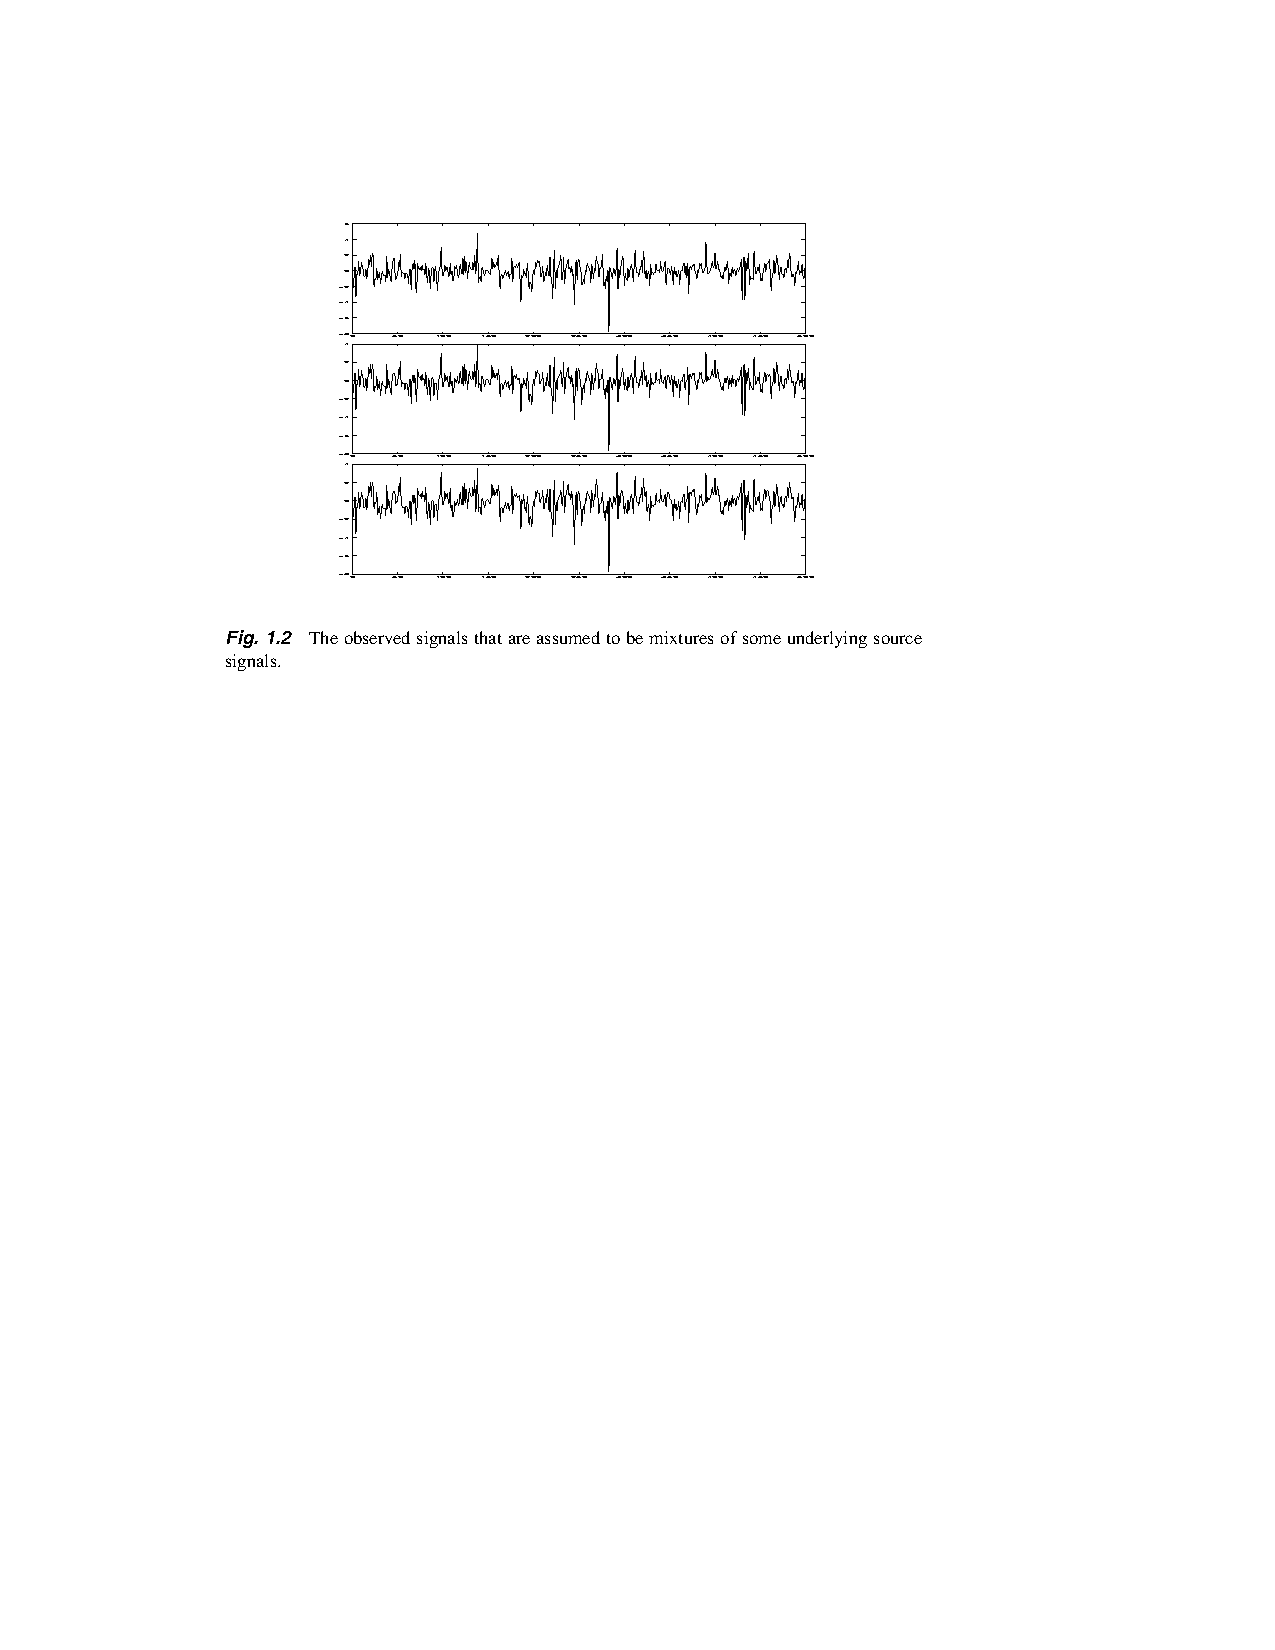
\includegraphics[width=0.7\textwidth]{ICABOOK2001_ObservedSignals} \\
				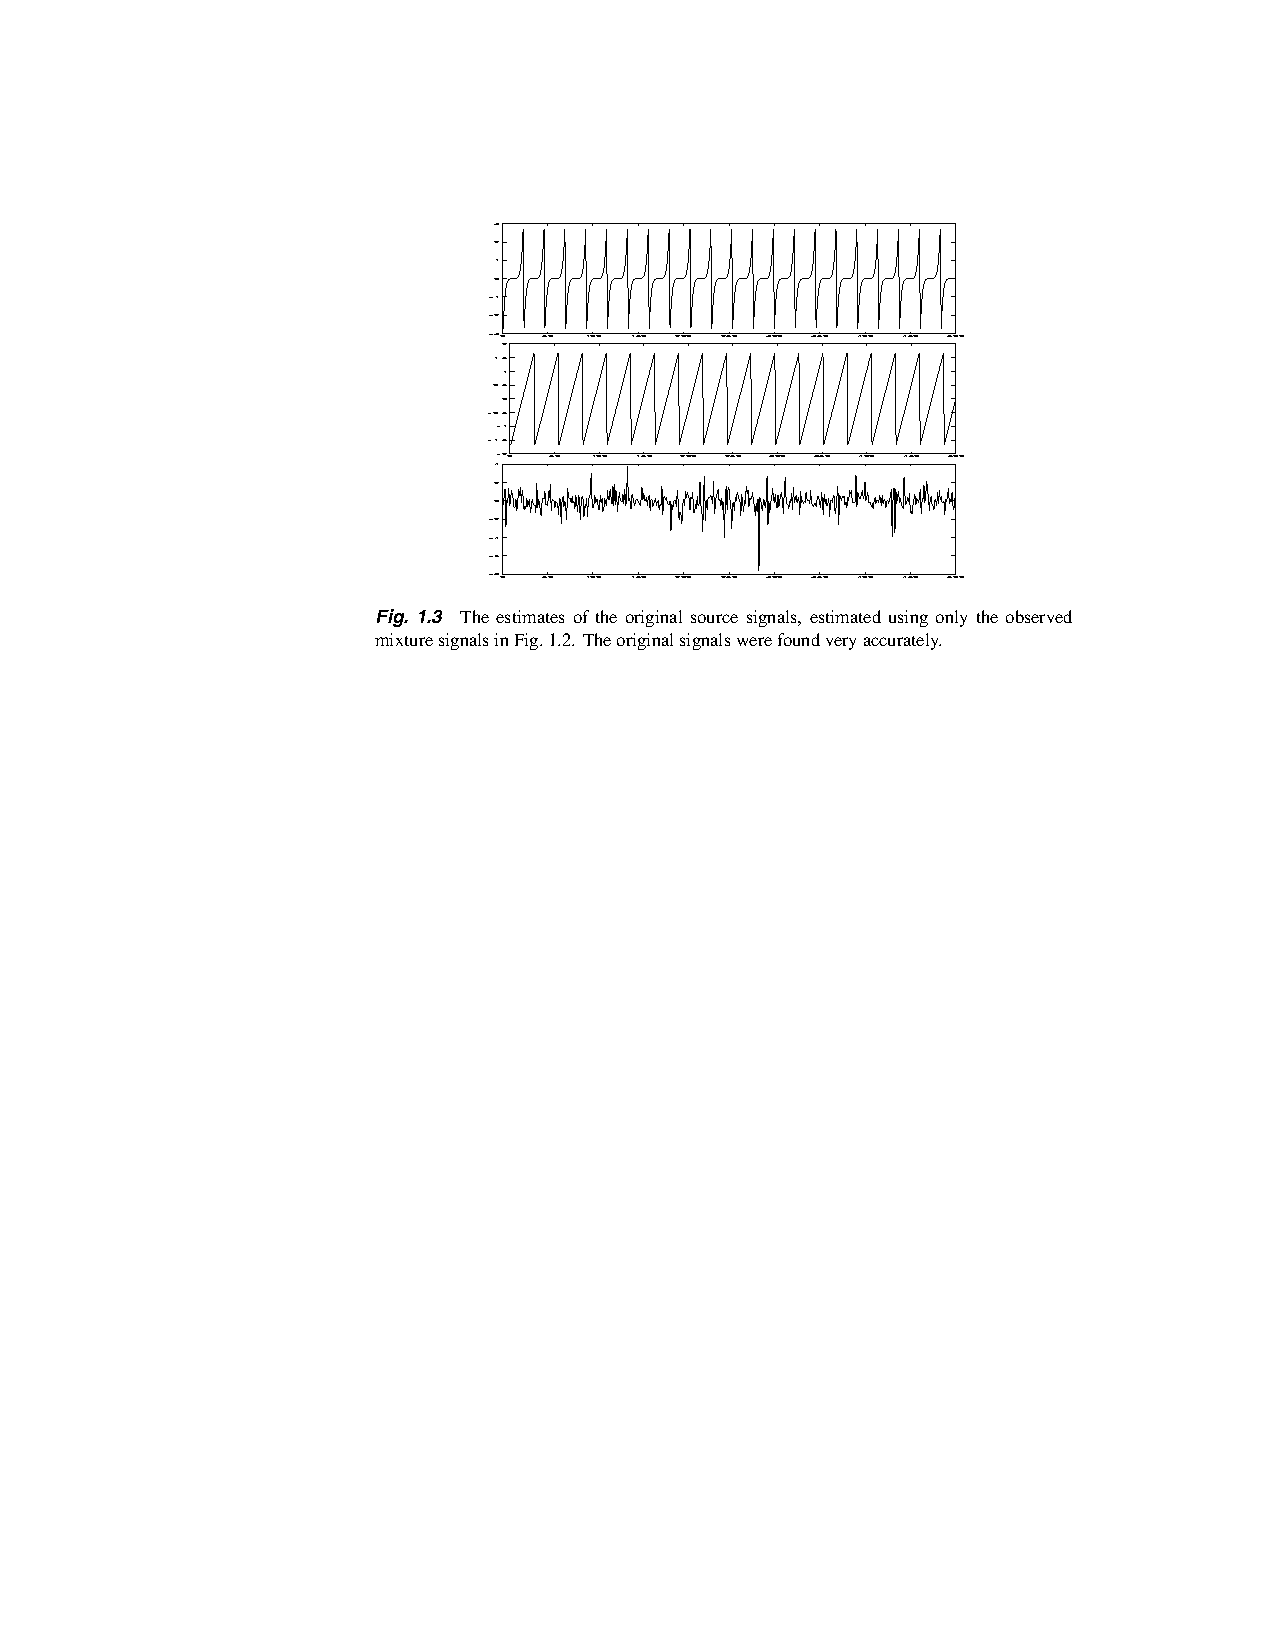
\includegraphics[width=0.7\textwidth]{ICABOOK2001_ReconstructedSignals}
				%\caption*{Behavior of various ICA methods}
			\end{figure}
			\vspace{-0.5cm} 					
		\end{block}
%		Deterministic signals
		\vspace{0.5ex}

	
		\begin{block}{Classical ICA}
		Given a set of observations of random variables
		$(x_1(t),x_2(t),\dots,x_d(t))$, 
		assume that they are generated as a linear mixture of \alert{independent components}:
		\[
		\begin{pmatrix}
		x_1(t)\\x_2(t)\\ \vdots \\ x_d(t)
		\end{pmatrix} = A
		\begin{pmatrix}
		s_1(t)\\s_2(t)\\ \vdots \\ s_d(t)
		\end{pmatrix}\,,
		\]
		where $A$ is some unknown matrix.
			\begin{itemize}
				\item $s = (s_1,\ldots, s_d)$ non-Gaussian, $\eps \sim \mathcal{N}(0,\Sigma)$ Gaussian random variables.
				\item Goal: Given $T$ independent observations $x(1), \ldots, x(T)$, reconstruct $A$ up to scaling and permutation.
				\item Assumptions:
                	\begin{itemize}
						\item $s_1(t),\ldots, s_d(t)$, $\eps_1(t), \ldots, \eps_d(t)$ are mutually independent for any $t$.
						\item $A$ is non-singular. (for simplicity). 
                     \end{itemize}				
			\end{itemize}
		\end{block}
		\vspace{0.5ex}
		\begin{block}{Independence?}
			\begin{itemize}
			\item Is $s_1(t)$ independent of $s_2(t)$? Sure!
			\item Any two numbers are independent of each other! 
			\alert{All deterministic signal sources are fine then?}
			\item Should we be worried about temporal dependencies? No? \alert{What if $s_1(t) = s_1(t+1) = \dots$?} 
			\item Can we redefine ICA in a more meaningful way?
			\item \alert{Let's go beyond statistics!}
			\end{itemize}
			\centering \vspace{0.5ex}
				{\large How? }
				\vspace{0.5ex}
			\begin{itemize}
				\item Perform a deterministic analysis of the algorithm, reducing the problem to perturbation analysis
				\item Perform statistical analysis on the size of perturbations when necessary or desired
			\end{itemize}
		\end{block}


	\end{column}
%------------------------------------------------------------------------------
% The second column
%------------------------------------------------------------------------------	
	\begin{column}{0.01\textwidth}
	\end{column}
	
	\begin{column}{.32\textwidth}% the right size for a 3-column layout
		\begin{block}{The Non-stochastic Setting}
			\begin{itemize}
				\item The source signals are a function of time: $s:[T] \to [-C,C]^d$.
				\item Empirical distribution induced by function $s$:
				\[
					\nu^{(s)}(B)=\tfrac{1}{t}|\{\tau \in [t]: s(\tau) \in B\}|.
				\]
				\item Measure of independence:
					\[
					D_4(\nu_1,\nu_2)	= \sup_{f\in\mathcal{F}} \big|\int f(s) \big(\nu_1(ds) -\nu_2(ds)\big) \big|,
					\]
				 $\mathcal{F}$: the set of all monomials up to degree $4$; 
				  \[ \quad D_4^{(p,q)} (\nu)= \inf_{\mu_1,\mu_2} D_4(\mu_1\otimes \mu_2,\nu).
				  \]
				  $\mu_1$ and $\mu_2$ range over all measures over $\real^p$ and $\real^q$.
				\item Measure Gaussianness:
					\begin{align*}
							\MoveEqLeft \kappa^2(\mu)  =   \max_{1\le i,j\le d} \sum_{k,l} 
							\big\{ 
							M_{i,j,k,l}(\mu) \\
							& - M_{i,j}(\mu) M_{k,l}(\mu) -  M_{i,k}(\mu) M_{j,l}(\mu) \\
							& - M_{i,l}(\mu) M_{j,k}(\mu)\big\}^2,
					\end{align*}
					where $M_{a,\dots,z}(\mu) = \int y_a \dots y_z \mu(dy)$.
				\item Measure of centrality: 
					\[
				 	N(\nu) = ||\int x \nu(dx) ||_F
					\]
				\item Accuracy of reconstruction:
					\[
					d(\hat{A},A) = \inf_{
						 \substack{\pi \in \mathrm{Perm}([d])\\
						 c\in \real^d}} \max_{k} 
						|| c_k A_{:\pi(k)} - A_{:k} ||_2\,.
					\]
			\end{itemize}
		\end{block}
		\vspace{0.5ex}
		\begin{block}{Main Result}
		\begin{center}
				\begin{tcolorbox}[title = \vspace{0.4cm}\textbf{\large Our Contributions} \vspace{0.4cm}, title filled, width = 0.95\textwidth, colback = uofagreen!10, colframe = red]
						\begin{itemize}
						\vspace{0.5cm}
						\item[$\diamondsuit$] Develop a randomized algorithm such that 
						for any $A\in \real^{d\times d}$, and $x, s, \eps: [T] \rightarrow \real^d$ satisfying $x(t) = As(t)+\eps(t)$,
						the algorithm returns $\hat{A}\in \real^{d \times d}$ such that:
							\begin{itemize}
								\item[--] The computational complexity is $O(d^3 T)$;
								\item[--] Universal: No free parameters;
								\item[--] With high probability, 
									\begin{align*}
									d(\hat{A}, A) & \le 
									\inf_{\mu\in \Pi_0} \mathcal{C}(\mu) \min\Big(D_4(\nu^{(s)},\mu) \\
									& + \kappa(\nu^{(\eps)}) + D_4^{(d,d)}(\nu^{(As,\eps)}) \\
										& +N(\nu^{(\eps)}) + N( \nu^{(s)}), \Theta(\mu) \Big);
									\end{align*}
								\item[] Here, $\mathcal{C}(\mu)$ and $\Theta(\mu)$ are problem dependent constants, polynomial in the parameters.
								\item[] $\Pi_0$ is the set of all product measures.
							\end{itemize}
						\vspace{1cm}
						\item[$\diamondsuit$] The above result covers
							\begin{itemize}
							\item[--] the classic stochastic setting;
							\item[--] Markov sources;
							\item[--] deterministic source signals.
							\item[]
							\end{itemize} 
						\end{itemize}	
					\vspace{0.5ex}	
				\end{tcolorbox}
		\end{center}				
		\end{block}
	\end{column}
%------------------------------------------------------------------------------
% The third column
%------------------------------------------------------------------------------

	\begin{column}{0.01\textwidth}
	\end{column}
	\begin{column}{0.32\textwidth}
			\begin{block}{Hsu and Kakade's method (HKICA)}
				\begin{figure}
				\begin{algorithmic}[1]
					\STATE Let $f(\eta) = \EEp{(\eta^{\top}x)^4} - 3 \EEp{(\eta^{\top}x)^2}^2$.
					\STATE  Choose $\phi$ and $\psi$. (How?)
					\STATE Let $T(\phi) = \nabla^2 f(\phi)$. Then 
						\[T(\phi) = AK \triangle\left( (\sigma_1,\ldots,  \sigma_d)\right)A^{\top},
						\]
						where $\sigma_i = \left(\phi^{\top}A_i\right)^2$ and $K$ is some diagonal matrix.
					\STATE Let $M = T(\phi)(T(\psi))^{-1}$. Then 
						\[M = A \triangle \left( \lambda_1, \ldots, \lambda_d \right) A^{-1},
						\]
						where $\lambda_i = \left(\frac{\phi^{\top}A_i}{\psi^{\top}A_i}\right)^2$.
					\STATE Do an eigen-decomposition of $M$ to recover $A$, assuming all $\lambda_i$'s are distinct.
				\end{algorithmic}
				\end{figure}
				\begin{itemize}
					\item Theoretical analysis shows that the performance depends on $\gamma_A^{-1}$,
					where
						\[
						\gamma_A = \min_{i\neq j} \left\vert \lambda_i - \lambda_j\right \vert.
						\]
					\vspace{-1cm}
					\item $\gamma_A$ is not yet well understood.
				\end{itemize}
			\end{block}
			\vspace{0.5ex}
		\begin{block}{Our method: Deterministic ICA (DICA)}		
			\begin{figure}
			\begin{algorithmic}[1]
				\STATE Sample $\psi$, $\phi_1$, and $\phi_2$ independently from standard normal distribution.
				\STATE Calculate $\nabla^2 f(\psi)$ and $B$ such that $\nabla^2 f(\psi) = BB^{\top}$.
				\STATE Calculate $T(\phi_1) = \nabla^2 f(B^{-\top}\phi_1)$ and $T(\phi_2) = \nabla^2 f(B^{-\top}\phi_2)$.
				\STATE Calculate $M = T(\phi_1)(T(\phi_2))^{-1}$.
					\[
					M = R \triangle\left( \tilde{\lambda}_1, \ldots, \tilde{\lambda}_d \right)R^{\top},
					\]
					where $\tilde{\lambda}_i = \left(\frac{\phi_1^{\top}R_i}{\phi_2^{\top}R_i}\right)^2$ and $R$ is some orthonormal matrix.
				\STATE Do an eigen-decomposition of $M$ to recover $R$.
				\STATE Return $\hat{A} = BR$ as an estimate of $A$. 
			\end{algorithmic}
			\end{figure}
			\begin{itemize}
				\item $\tilde{\lambda}$ (and its minimal gap) is now independent of $A$, and easier to analyze.
				\item Simulation results are provided in the paper.
			\end{itemize}
		\end{block}
		\vspace{0.5ex}
		\begin{block}{Conclusions}
		\begin{itemize}
		\item Independent Component Analysis without probabilities! 
		\item Deterministic analysis: Cleaner, more general, should do it more often! Limits?
		\item New method: DICA. Universal, strong guarantees.
		\end{itemize}
		\end{block}
		\vspace{0.5ex}
		\begin{block}{Acknowledgements}
This work was supported by Alberta Innovates Technology Futures and NSERC.
		\end{block}
	\end{column}
		
	\begin{column}{0.01\textwidth}
	\end{column}
\end{columns}
 
\end{frame}

\end{document}
